\documentclass[11pt]{article}
\usepackage[preprint]{acl}
% compile with xelatex: the Kazakh letters need a Unicode font
\usepackage{fontspec}
\setmainfont{Times New Roman}
\setmonofont{Consolas}[Scale=0.9]
\usepackage{latexsym}
\usepackage{microtype}
\usepackage{graphicx}
\usepackage{booktabs}
\usepackage{multirow}
\graphicspath{{../../results/figures/}}

\newcommand{\ru}[1]{#1}

\title{Do Retrievers Confuse ``May'' and ``May Not''?\\
A Parallel Russian--Kazakh Benchmark for Negation in Legal Retrieval}

\author{Maxim Abakarov \and Balym Sekenova \\
  Kazakh-British Technical University}

\begin{document}
\maketitle

\begin{abstract}
A retrieval-augmented legal assistant answers from the articles its retriever returns. If the retriever
returns a norm with the opposite polarity (``the employer may'' instead of ``the employer may not''), the
answer contradicts the law. We study this failure for Russian and Kazakh, where Kazakh marks negation with a
verbal affix. We build a parallel corpus of 22 codes of the Republic of Kazakhstan (30,766 aligned chunks per
language) and 49 parallel question pairs on the Labor and Tax Codes, each with a gold paragraph and, for
polarity-sensitive questions, an opposite-polarity ``twin''. We test two inexpensive fixes against controls:
BM25 that keeps negation as a token, fused with a dense retriever, and a fine-tuned NLI reranker. With
19 or 20 test questions per slice the study has little power: no difference survives an exact sign test
with a Holm correction, so we report the results as a pilot. With bge-m3 the dense retriever alone puts a
twin above the gold for 2 of 14 Russian and 1 of 14 Kazakh questions (Wilson intervals [0.04, 0.40] and
[0.01, 0.31]). The NLI reranker is not better than off-the-shelf cross-encoder rerankers in any setting.
The negation token in BM25 changes almost nothing: it occurs in 43--45\% of all chunks. Where the hybrid
helps a weaker retriever (multilingual-e5-base on Kazakh, Recall@5 on polarity-sensitive questions 0.47 to
0.68, 4 questions changed), the gain comes from lemmatization. Fine-tuning the NLI model on rule-generated
legal pairs raises its accuracy on held-out synthetic pairs from 0.68 to 0.97 with no detectable gain on
hand-written pairs. We release the corpus, questions, diagnostics and code at
\url{https://github.com/ixlander/kz-legal-negation-ir}.
\end{abstract}

\section{Introduction}

Legal question answering systems increasingly retrieve statutes and generate an answer from them.
Retrieval does not remove errors: commercial legal research tools built this way gave hallucinated answers in
17\% to 33\% of the queries in a preregistered evaluation \citep{magesh2024hallucination}. One source of such
errors is negation. A norm and its negation differ by one word, and embedding models place them close
together. On the NevIR benchmark \citep{weller-etal-2024-nevir} most bi-encoders score between 6.5\% and 22.6\% pairwise accuracy, below
the 25\% of random ranking, while a multilingual cross-encoder reranker (jina-reranker-v2) reaches 65.2\%
\citep{vandenelsen2025nevir}.

We ask whether this failure appears in statutory retrieval for Russian and Kazakh, and whether two cheap
components fix it. Kazakh is of interest because it marks negation inside the verb (\ru{төлейді} ``pays'',
\ru{төлемейді} ``does not pay''), and a subword tokenizer may not keep the negative affix as a unit, as
reported for the Turkish negative suffix by \citet{toraman2023tokenization}. There is no legal retrieval
benchmark for Kazakh that we know of.

Our research question is: do a morphology-aware BM25 and an NLI reranker retrieve the article with the right
polarity, and do they help Kazakh more than Russian? The contributions are:

\begin{enumerate}
\item A parallel Russian--Kazakh corpus of 22 codes of Kazakhstan, split into paragraphs and aligned, and 49
question pairs with gold and twin paragraphs, checked by a native speaker of Kazakh.
\item Two diagnostics of encoders before retrieval (Negation Margin, Affix Isolation Rate) and two
retrieval metrics for polarity errors (Negation Gap, Twin-above-Gold).
\item An ablation from dense retrieval to hybrid retrieval to reranking, with an off-the-shelf reranker and a
polarity rule as controls, paired bootstrap intervals, control runs and an error analysis.
\end{enumerate}

The hypotheses were fixed before the evaluation set was finished and are reported with their outcome, most
of which are negative.

\section{Related work}

\paragraph{Negation in retrieval.} \citet{vandenelsen2025nevir} reproduce NevIR \citep{weller-etal-2024-nevir}, where each query pair has
two documents that differ by negation, and extend it to LLM-based rerankers. Cross-encoders do much better
than bi-encoders, and fine-tuning on NevIR raises a cross-encoder to about 75\% but can lower results on
MS~MARCO. They also find that only cross-encoders transfer between NevIR and ExcluIR. NevIR is English and
general-domain; our twins are real norms from the same code, not constructed edits.

\paragraph{Legal retrieval and entailment.} The COLIEE competition pairs statute retrieval with statute
entailment. \citet{kim2024coliee} fine-tune DeBERTa trained on SNLI and MultiNLI for the entailment task.
We use an NLI model as a reranker over retrieval candidates. BSARD \citep{louis-spanakis-2022-statutory} is a
statutory article retrieval dataset with legal questions over Belgian law articles in French; our set is
smaller but parallel in two languages and marks opposite-polarity twins. \citet{chi2026legalai} survey LLM roles in legal
classification, retrieval and generation, and \citet{ren2026legal} combine synthetic legal data with
retrieval-augmented generation. All of these study English or Chinese.

\paragraph{Morphology of Turkic languages.} \citet{toraman2023tokenization} compare tokenizers for Turkish
and find a morphological tokenizer competitive with BPE and WordPiece. \citet{tukeyev2026kazakh} report gains
from morphology-aware normalization for Kazakh question answering in programming education. We measure how
often multilingual tokenizers isolate the Kazakh negative affix and whether a morphological BM25 changes
retrieval.

\section{Data}

\subsection{Corpus}
We downloaded all codes in force from adilet.zan.kz, the official legal database of Kazakhstan, whose Russian
and Kazakh versions have the same revision date: 22 codes (the Entrepreneurial Code was excluded because its
two versions differ). Articles are split into paragraphs; long paragraphs without numbered points are split
into groups of sub-points. The article title is prepended to each chunk. This gives 30,766 chunks per
language. Questions are asked only about the Labor and Tax Codes; the other 20 codes are distractors.

Russian and Kazakh chunks share an id (code, article, paragraph). We checked alignment automatically for all
pairs: paragraph numbering agrees in 99.7\% and the numbers in the text in 99.4\%. A native speaker reviewed
18 flagged pairs and rejected 7. One rejection is a finding about the source: in Article 26 of the Kazakh
Labor Code, points 1 and 2 appear in the reverse order.

\subsection{Questions}
Questions were drafted in Russian with an LLM assistant, translated into Kazakh, and checked by a native
speaker of Kazakh together with their gold and twin ids. 49 of 50 pairs were accepted (one was dropped
because its gold paragraph is one of the misaligned ones). A question is in the \emph{negation} slice if a
retriever that confuses polarity would lead to the wrong answer (``May an employer dismiss a pregnant
employee due to staff reduction?''), and in the \emph{general} slice otherwise (``What is the standard VAT
rate?''). For negation questions the annotator marked a twin: a paragraph on the same topic with the
opposite polarity, if the code has one. Each language has 25 general and 24 negation questions; 5 pairs per
slice form a dev split used for tuning, the remaining 20 general and 19 negation pairs form the test split.
14 of the 19 test negation questions have a twin.

\paragraph{How the questions were checked.} We state the protocol in full because it limits what the
check shows. The annotator saw the LLM drafts and the proposed gold and twin ids. She accepted 49 of the 50
pairs without editing the question, the Kazakh version, the gold or the twin; the save times of the review
page give a median of 17 seconds between consecutive question cards. The final test questions are therefore
the drafts word for word. Two drafts had their gold corrected before annotation, after a retrieval run on the
drafts showed that the gold pointed to the wrong paragraph (tax\_001/002: article 382(5), with 383(1) and
384(1) as twins). The design of the NLI reranker (the fusion with the retrieval order and the grids for
$\lambda$ and $\alpha$) was developed on the same draft questions before the dev/test split was drawn. In 14
of the 25 Russian Tax questions the drafts use the abbreviations for VAT, personal and corporate income tax
(\ru{НДС, ИПН, КПН}), while the Kazakh versions and the code text spell the terms out; \ru{ИПН} does not occur in
the Tax Code at all.

\subsection{NLI data}
For the NLI reranker we sampled 50,000 pairs each from the Russian and Turkish training sets of XNLI
\citep{conneau-etal-2018-xnli} and from a machine-translated Kazakh SNLI \citep{bowman-etal-2015-large}
(the Hugging Face dataset \texttt{sultanbi/snli-kazakh}). We also generated synthetic pairs from the 20 distractor codes, so
that no Labor or Tax Code text enters training: polarity flips and modality swaps as contradictions
(\ru{вправе} $\rightarrow$ \ru{не вправе}), negated ranges and synonymous negatives as entailments
(\ru{не менее} $\rightarrow$ \ru{не меньше}), and tighter or looser numeric bounds as neutral or entailment
pairs. This gives 3,708 Russian and 2,901 Kazakh pairs; 10\% of the articles are held out as a synthetic test
set. For validation we use the Kazakh XNLI of Karde\c{s}-NLU \citep{senel-etal-2024-kardes} (post-edited by native
speakers), the Russian RCB and LiDiRus sets of RussianSuperGLUE \citep{shavrina-etal-2020-russiansuperglue}, and a hand-written set of 50 Russian and 50 Kazakh pairs whose premises are verbatim
Labor or Tax Code norms and whose hypotheses were written without the templates of the generator. 21 pairs per
language contain ``not less than'', ``not more than'' or ``not later than''. The annotator changed 3 of the 50
draft labels (6\%). On re-reading, all three changes go against the annotation guideline (pairs v019, v030,
v035: two contradictions and one neutral pair relabelled as entailment), so we also report results without
these pairs.

\section{Metrics}

\paragraph{Negation Margin (D1).} For a legal sentence $s$, a paraphrase $p$ and its negation $n$:
$\cos(s,p) - \cos(s,n)$. A negative value means the negation is closer than the paraphrase. As a control we
replace the paraphrase with a one-word synonym edit $m$, so that both alternatives differ from $s$ by about
one word: $\cos(s,m) - \cos(s,n)$. 30 sentence triples per language. In 4 Kazakh triples the annotator's
correction made $m$ identical to $s$; these are left out of the control, which uses 26 Kazakh triples.

\paragraph{Affix Isolation Rate (D2).} The share of Kazakh negative verb forms in which the tokenizer puts a
token boundary both before and after the negative affix (\ru{-ма/-ме/-ба/-бе/-па/-пе}). 171 forms from the
Labor Code; 154 were confirmed by two morphological analyzers (kaznlp\footnote{\url{https://github.com/nlacslab/kaznlp}}
and apertium-kaz\footnote{\url{https://github.com/apertium/apertium-kaz}}) and 17 by the annotator. We report it for
the XLM-R tokenizer \citep{conneau-etal-2020-unsupervised} and 13 other tokenizers.

\paragraph{Retrieval.} Recall@5 over the full 22-code corpus; \emph{Negation Gap} = Recall@5(general) $-$
Recall@5(negation); \emph{Twin-above-Gold} (TaG) = the share of negation questions with a twin where the best
twin ranks above the best gold in the full ranking. Because a full-ranking TaG also counts cases where both
paragraphs are far down the list, we also report TaG@5 (the twin is in the top 5 and above the gold) and the
polarity miss (the twin is in the top 5 and the gold is not). One question changes Recall@5 by 0.05 and TaG by
0.07. Differences are estimated with a paired bootstrap over questions (1,000 resamples, seed 42, 95\%
percentile interval) and tested with an exact two-sided sign test on the questions that changed, with a Holm
correction over the 40 pre-registered comparisons of H1--H3. Absolute rates get Wilson intervals.

\section{Systems}

\begin{description}
\item[B0] Dense retrieval. Main model bge-m3 \citep{chen2024m3}; multilingual-e5-base \citep{wang2024multilingual}
(with \texttt{query:}/\texttt{passage:} prefixes) for comparison. Cosine similarity over all chunks.
\item[B1] B0 fused with BM25 \citep{robertson2009prf} over lowercased word tokens by reciprocal rank fusion
(RRF, $k=60$; \citealp{cormack2009rrf}).
\item[B2] B0 fused with a morphological BM25. Russian: pymorphy3 lemmas \citep{korobov2015pymorphy2}, function words removed except
\ru{не, ни, нет, без}, a fused negative prefix split off (\ru{неуплата} $\rightarrow$ \ru{не уплата}).
Kazakh: kazsearch\footnote{\url{https://github.com/iDynbek/kazsearch-py}} stems, negative verb forms split into stem plus a \texttt{NEG} token by a regular
expression that checks vowel harmony and consonant assimilation, \ru{емес} and \ru{жоқ} kept.
\item[B3$'$] The top 30 of B2 reordered by an off-the-shelf cross-encoder: jina-reranker-v2-base-multilingual\footnote{\url{https://huggingface.co/jinaai/jina-reranker-v2-base-multilingual}}
or bge-reranker-v2-m3\footnote{\url{https://huggingface.co/BAAI/bge-reranker-v2-m3}}. As a follow-up we also rerank the top 30 of B0.
\item[B3-rule] The top 30 of B2 with $\pm\alpha$ added to the score when the polarity of the chunk sentence
with the largest word overlap does (or does not) match the polarity of the question.
\item[B3] The top 30 of B2 reordered by an NLI model with the chunk as premise and the question as hypothesis.
Scores $S1 = P(e) - P(c)$ or $S2 = P(e) + P(c)$, used alone, fused with the B2 order by RRF, or added to the
normalized B2 score with weight $\lambda \in \{0.25, 0.5, 1\}$.
\end{description}

The NLI model is mDeBERTa-v3-base-xnli-multilingual-nli-2mil7 \citep{laurer2022less}, built on mDeBERTa-v3
\citep{he2023debertav3}, fine-tuned for two epochs (learning rate
$10^{-5}$, batch 32, bf16) in four variants: (a) XNLI ru + tr + synthetic, 105,986 pairs; (b) a without
Turkish; (c) a without the synthetic entailment counter-examples; (d) a plus SNLI-kk. We first trained
XLM-R-base from scratch on variant a; it was worse than the off-the-shelf mDeBERTa model on every validation
set (Karde\c{s} 0.71 vs.\ 0.79) and almost always predicted neutral on the hand-written pairs, so we switched
the base model. The epoch is chosen on the even half of the Karde\c{s} test set and results are reported on the
odd half; the Karde\c{s} dev set is not used because it translates the XNLI validation set on which the base
model was trained. $\alpha$ for B3-rule and the scoring and fusion of B3 are chosen on dev by mean Recall@5
over both slices and both languages. The NLI model reads at most 256 tokens of premise and hypothesis and was
trained at 128, while the cross-encoders read 512; 16 of the 66 Russian and 18 of the 66 Kazakh gold and twin
chunks are longer than 256 tokens. The control runs in Section~6.4 were added after the test results were
known and are exploratory.

\section{Results}

\subsection{Sanity checks against published numbers}
On RuLawRetrieval \citep{rulawretrieval2026} (split tk\_hard, 716 queries) our pipeline gives nDCG@10 of 0.839 for bge-m3, 0.762 for
multilingual-e5-base and 0.501 for our Russian BM25; the dataset card reports 0.820 for e5-large, 0.710 for
e5-small and 0.480 for BM25. On NevIR our jina-reranker-v2 gives 0.651 pairwise accuracy against the
published 0.652; this is the only like-for-like comparison, the RuLawRetrieval figures are for other models
and serve as a range. On a 52,660-passage subsample of KazQAD \citep{yeshpanov-etal-2024-kazqad} (1,929 test questions) our Kazakh analyzer raises
BM25 from 0.348 to 0.465 nDCG@10; bge-m3 reaches 0.606 and e5-base 0.493.

\subsection{Diagnostics}

\begin{table}[t]
\centering\small\setlength{\tabcolsep}{4pt}
\begin{tabular}{lrrrr}
\toprule
& \multicolumn{2}{c}{vs.\ paraphrase} & \multicolumn{2}{c}{vs.\ one-word edit} \\
Model & ru & kz & ru & kz \\
\midrule
e5-base & $-$.018 & $-$.013 & .018 & .025 \\
e5-large-instruct & $-$.004 & $-$.019 & .028 & .014 \\
bge-m3 & $-$.008 & $-$.013 & .099 & .092 \\
LaBSE & $-$.073 & $-$.072 & .033 & .042 \\
Qwen3-Emb-0.6B & $-$.122 & $-$.169 & .030 & .023 \\
EmbeddingGemma & $-$.065 & $-$.088 & .005 & $-$.004 \\
\bottomrule
\end{tabular}
\caption{Mean Negation Margin over 30 triples per language (Kazakh control: 26). Left: margin against a full
paraphrase. Right: the control, margin against a one-word synonym edit. Negative: the negation is closer.}
\label{tab:d1}
\end{table}

\paragraph{D1.} Against a full paraphrase the margin is negative for all six encoders in both languages
(Table~\ref{tab:d1}; besides bge-m3 and e5 the pool has LaBSE \citep{feng-etal-2022-language}, Qwen3-Embedding
\citep{zhang2025qwen3} and EmbeddingGemma \citep{vera2025embeddinggemma}); for e5-base the negation is closer than the paraphrase for 90\% of the Russian and
80\% of the Kazakh norms. For bge-m3 the interval includes zero (Russian $-0.008$ [$-0.036$, $0.020$]). The
paraphrase changes about 20 words and the negation about one, so this comparison mixes negation with edit
size. Against a one-word synonym edit the margin is positive with an interval above zero for all six encoders
in Russian and for five in Kazakh (e5-base Russian $0.018$ [$0.013$, $0.022$]); EmbeddingGemma on Kazakh is the
exception ($-0.004$ [$-0.009$, $0.000$]). The encoders do separate a negation from a synonym, by 0.01 to 0.10
cosine. D1 compares passages with edited passages; we did not measure the retrieval analogue,
$\cos(q, \mathrm{gold}) - \cos(q, \mathrm{twin})$.

\paragraph{D2.} The XLM-R tokenizer, shared by e5 and bge-m3, isolates the negative affix in 21.1\% of the
171 forms and puts at least one boundary at the affix in 95.9\%. Across 14 tokenizers the rate ranges from
0\% (five Kazakh monolingual tokenizers, which keep frequent negative forms as one token) to 49.7\% (mBERT).
We report D2 as a description: isolating the affix is neither necessary nor sufficient for a contextual
encoder to represent negation. We see no sign that it hurts retrieval: bge-m3 with this tokenizer has
Recall@5 0.97 on Kazakh negation questions and 0.79 on Russian ones. This comparison is confounded by the
abbreviations in the Russian questions: on the 11 test pairs whose Russian question has one, bge-m3 finds the
gold in the top 5 for 7 Russian and 10 Kazakh questions; on the other 28 pairs, for 27 and 28.

\subsection{Retrieval}

\begin{table*}[t]
\centering\small
\begin{tabular}{llrrrrrr}
\toprule
& & \multicolumn{3}{c}{Russian} & \multicolumn{3}{c}{Kazakh} \\
Model & Run & gen R@5 & neg R@5 & TaG $\downarrow$ & gen R@5 & neg R@5 & TaG $\downarrow$ \\
\midrule
\multirow{6}{*}{bge-m3}
& B0 dense & .95 & .79 & .14 & .95 & .97 & .07 \\
& B1 + BM25 & .80 & .58 & .36 & .80 & .74 & .14 \\
& B2 + morph.\ BM25 & .85 & .74 & .21 & .90 & .89 & .07 \\
& B3$'$ jina-v2 & .93 & .84 & .07 & .90 & .92 & .07 \\
& B3$'$ bge-reranker & 1.00 & .84 & .07 & .95 & .92 & .00 \\
& B3 NLI ($S1$, lin.\ 0.25) & .90 & .74 & .36 & .90 & .89 & .07 \\
\midrule
\multirow{6}{*}{e5-base}
& B0 dense & .93 & .74 & .29 & .78 & .47 & .43 \\
& B1 + BM25 & .72 & .68 & .36 & .85 & .58 & .36 \\
& B2 + morph.\ BM25 & .82 & .68 & .21 & .90 & .68 & .14 \\
& B3$'$ jina-v2 & .97 & .84 & .07 & .90 & .84 & .14 \\
& B3$'$ bge-reranker & 1.00 & .89 & .07 & .95 & .89 & .07 \\
& B3 NLI ($S2$, RRF) & .88 & .79 & .21 & .85 & .63 & .21 \\
\bottomrule
\end{tabular}
\caption{Test split: 20 general and 19 negation questions per language, Twin-above-Gold over the 14 negation
questions with a twin. B3-rule is omitted: dev selected $\alpha=0$ for both models, which makes it identical
to B2. B3 scoring was selected on dev separately for each dense model. Recall@5 can be fractional because two
questions have two gold paragraphs.}
\label{tab:main}
\end{table*}

\begin{figure*}[t]
\centering
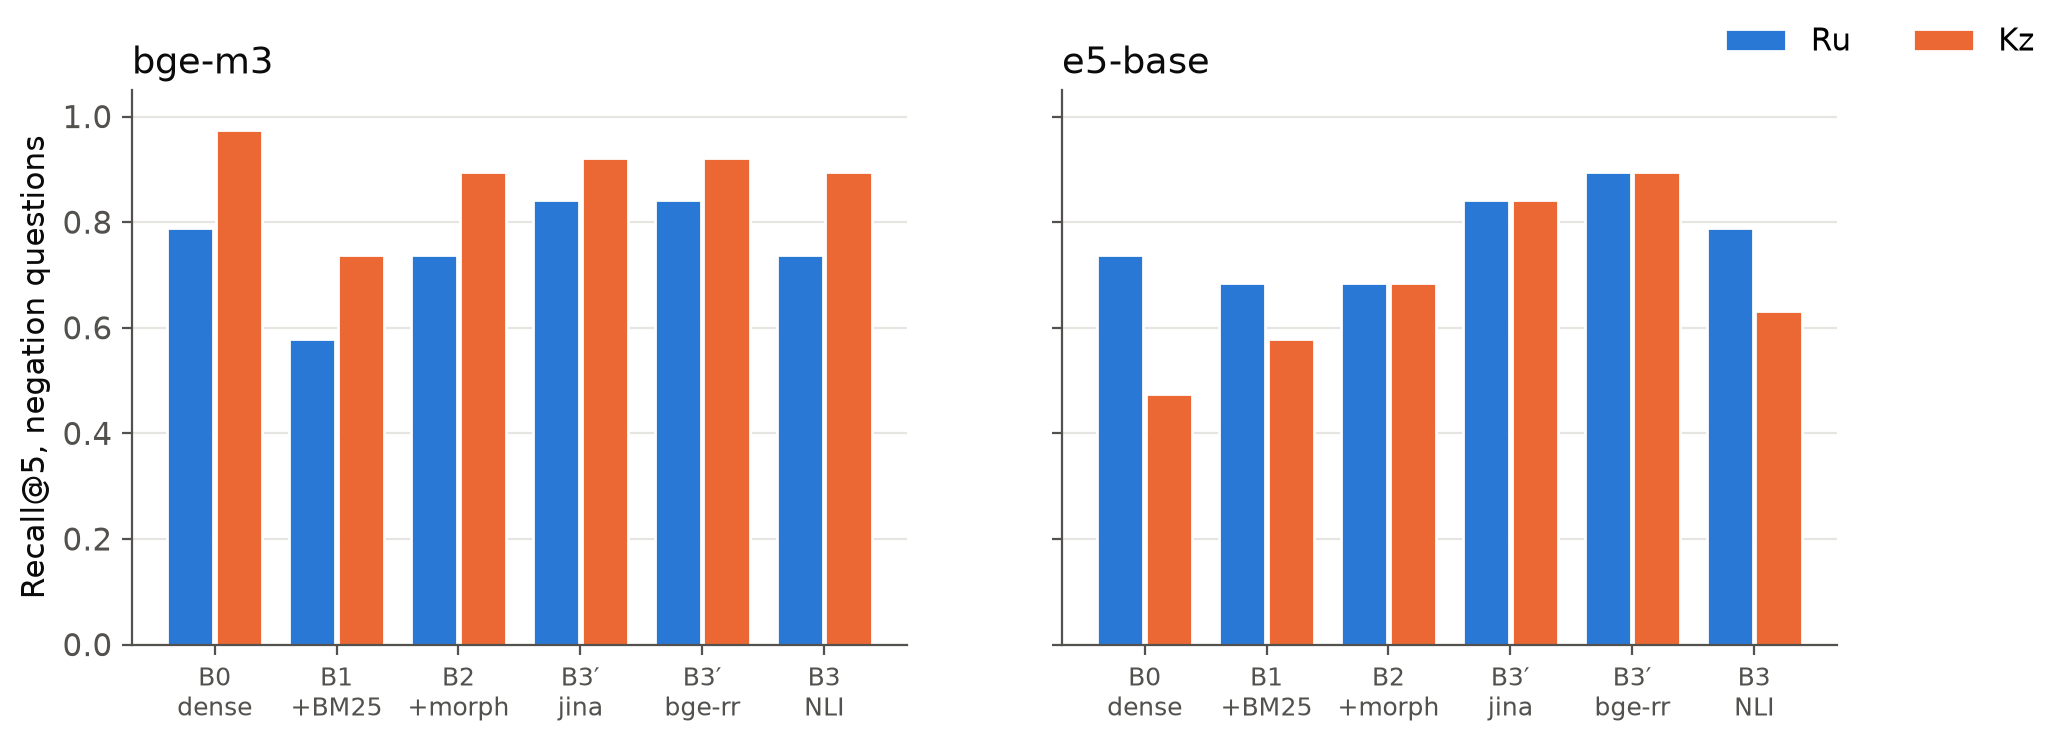
\includegraphics[width=0.82\textwidth]{ladder_negation_r5.png}
\caption{Recall@5 on negation questions on the test split, by configuration, language and dense model
(19 questions per language). Twin-above-Gold for the same runs is in Table~\ref{tab:main}.}
\label{fig:ladder}
\end{figure*}

Table~\ref{tab:main} and Figure~\ref{fig:ladder} show the test results. Five of the tested differences have
a bootstrap interval that excludes zero. Each rests on 4 or 5 questions that all changed in the same direction;
the exact sign test gives $p = 0.06$ to $0.13$ for each, and none remains below 0.05 after the Holm correction.
We read them as suggestive.

\paragraph{H1: the morphological BM25 does not reduce the Negation Gap.} For both models and both languages
the change of the gap from B0 to B2 is within the interval (bge-m3 Russian $-0.05$ [$-0.25$, $0.16$], e5-base
Kazakh $-0.09$ [$-0.37$, $0.19$]). For e5-base on Kazakh, B2 raises Recall@5 on negation questions from 0.47 to
0.68 ($+0.21$ [$0.05$, $0.42$]; 4 questions gained, none lost, $p = 0.13$); general questions also rise, from 0.78 to 0.90, within the interval. For
bge-m3, B2 has lower Recall@5 than B0 in all four cells, without a found difference.

\paragraph{H2: the NLI reranker is not better than the controls.} B3 is never above an off-the-shelf
reranker. With e5-base on Kazakh it is below both on negation Recall@5 (vs.\ jina $-0.21$ [$-0.42$,
$-0.05$], vs.\ bge-reranker $-0.26$ [$-0.47$, $-0.11$]), and with bge-m3 on Russian its TaG is higher than
that of bge-reranker ($+0.29$ [$0.07$, $0.54$], 4 questions). The last difference follows partly from the
selected score $S1 = P(e) - P(c)$: in 22 of the 24 Russian negation questions the gold is a prohibition, and
a prohibition contradicts a positively phrased question. Even the B3 variant that is best on test (mean
Recall@5 0.87 for bge-m3, 0.83 for e5-base) is below bge-reranker (0.93 and 0.94), so H2 does not depend on
the noisy dev selection. The polarity rule could not be tested as intended: on dev $\alpha = 0.002$ tied
with $\alpha = 0$ and larger values lowered recall, because almost no question contains a negation word (in
Russian, 1 of 24 contains \ru{не}; 4 contain any negation token of the analyzer) while 22 of the 24 gold
paragraphs contain one.

\paragraph{H3: a larger Kazakh gain only for the weaker model.} For e5-base, the B2 gain on negation questions
is larger for Kazakh than for Russian by $0.26$ [$0.11$, $0.47$] (19 pairs). The gain on general questions is
of similar size ($0.23$ [$-0.03$, $0.53$]), so we read this as lexical matching helping a weaker Kazakh dense
model, not as an effect specific to negation. The Kazakh baseline also has more room to improve (0.47 vs.\
0.74). For bge-m3 we find no difference.

\subsection{Control runs}
\paragraph{Negation tokens in BM25.} Removing the negation tokens (\ru{не, ни, нет, без}; \texttt{NEG},
\ru{емес}, \ru{жоқ}) from the index and the queries leaves BM25 alone unchanged (Recall@5 0.58 Russian, 0.77
Kazakh) and leaves B2 unchanged for bge-m3 in both languages and for e5-base on Kazakh. For e5-base on Russian
the version without negation tokens is slightly better (general $0.88$ vs.\ $0.82$). The gain of B2 over B1
comes from lemmatization and stemming. Two facts explain this. Few questions contain a negation word, and a
negation token that is not bound to its predicate cannot separate ``taxable'' from ``not taxable'' on the
same topic: \ru{не} occurs in 44.9\% of the Russian chunks and \texttt{NEG} in 42.5\% of the Kazakh ones, which
gives them a BM25 IDF of 0.80 and 0.86 against 4--8 for typical content words.

\paragraph{Fusion weight.} With equal weights, B2 is below B0 for bge-m3. With the BM25 weight set to 0.25 and
each ranking cut at its top 1,000, the hybrid is not below B0 in any cell (Russian general 1.00 vs.\ 0.95,
Kazakh TaG 0.00 vs.\ 0.07), and not significantly above it. For e5-base dev selects a BM25 weight of 2; with 10
dev pairs we report the weights as a sensitivity analysis.

\paragraph{Reranking the dense top 30.} The rerankers in Table~\ref{tab:main} reorder the hybrid's top 30.
Reordering the top 30 of B0 instead, bge-reranker raises bge-m3's negation Recall@5 on Russian from 0.79 to
0.92 ($+0.13$ [$0.00$, $0.29$]) and leaves Kazakh at 0.92 vs.\ 0.97 for B0; TaG becomes 0.07 and 0.00. For
e5-base on Kazakh the dense top 30 misses many golds, and reranking it gives 0.63, against 0.89 over the hybrid
($-0.26$ [$-0.47$, $-0.05$]). The candidate pool matters more than the reranker for the weaker retriever.

\paragraph{Abbreviations written out.} Replacing \ru{НДС, ИПН, КПН} in the Russian questions by the full
terms moves most cells by one or two questions in either direction (at most three) and no difference is found (bge-m3 B0 negation
$+0.05$ [$0.00$, $0.16$], B2 $-0.05$ [$-0.16$, $0.00$]).

\paragraph{NLI without fine-tuning and questions as statements.} Using the base mDeBERTa model in B3 gives the
same results as the fine-tuned model: mean Recall@5 over the ten scoring and fusion variants 0.80 vs.\ 0.81
(bge-m3) and 0.74 vs.\ 0.76 (e5-base), mean TaG 0.21 vs.\ 0.20 and 0.24 vs.\ 0.24. Both are below B2 on average
(0.85 and 0.77). Turning yes/no questions into statements by removing the question particle lowers mean
Recall@5 to 0.70 (base model, bge-m3).

\subsection{NLI models}

\begin{table}[t]
\centering\small\setlength{\tabcolsep}{4pt}
\begin{tabular}{lrrrr}
\toprule
Model & Kard.\ kk & man.\ ru & man.\ kz & syn.\ ru \\
\midrule
base & .779 & .62 & .56 & .675 \\
a: ru+tr+synth & .807 & .56 & .48 & .972 \\
b: a $-$ tr & .812 & .64 & .50 & .974 \\
c: a $-$ counter-ex. & .797 & .40 & .40 & .647 \\
d: a + SNLI-kk & .801 & .50 & .44 & .972 \\
\bottomrule
\end{tabular}
\caption{NLI accuracy: Karde\c{s}-NLU Kazakh test (odd half, 1,000 pairs), manual hand-written legal pairs (50 per
language), held-out synthetic Russian pairs (351).}
\label{tab:nli}
\end{table}

Fine-tuning raises accuracy on Karde\c{s} by 0.02 to 0.03 (a vs.\ base $+0.028$ [$0.009$, $0.048$]) and on
the held-out synthetic pairs from 0.68 to 0.97 (Table~\ref{tab:nli}). On the hand-written legal pairs the point
estimates go down, but no difference is found: a vs.\ base $-0.06$ [$-0.20$, $0.06$] in Russian and $-0.08$
[$-0.22$, $0.04$] in Kazakh, and the same holds without the three doubtful labels (base 0.66 and 0.60, a 0.60
and 0.51 on 47 pairs). The synthetic test shares its rewrite templates with training, so we read the 0.97 as
template learning.

\paragraph{H5: Turkish data.} Variants a and b do not differ on Karde\c{s} ($+0.005$ [$-0.010$, $0.019$]) or
on the Kazakh hand-written pairs ($+0.02$ [$-0.04$, $0.08$]). On the Russian hand-written pairs the variant
without Turkish is better ($+0.08$ [$0.02$, $0.16$]). The comparison is weak for two reasons: the base
model was already trained on machine-translated NLI data in 26 languages that include Russian and Turkish but
not Kazakh (105,000 pairs per language, according to its model card), and variant b has about half the
training data of a.

\paragraph{H6: entailment counter-examples.} On the 110 Russian synthetic test entailments with a negated range
or a numeric bound, the base model calls 35.5\% contradictions, variant a 0.9\% and variant c (without
counter-examples) 60.9\%; both differences to the base model have intervals that exclude zero. On these
in-distribution pairs the counter-examples do what H6 predicts. On hand-written pairs the evidence is too thin:
of the 8 Kazakh range entailments with an undisputed label the base model calls 3 contradictions and both a and
c call none (c labels them neutral), so the drop cannot be attributed to the counter-examples. We consider H6
supported on synthetic data and untested on human-written data.

\subsection{Error analysis}
We took the 20 test questions with the most Recall@5 misses over five runs (bge-m3 B0, B2, B3$'$ with
bge-reranker; e5-base B0, B2) and assigned each a cause by reading the top-ranked chunks; the categories were
assigned by us with an LLM assistant and not checked by a second person. Seven are e5-base
failures on Kazakh where bge-m3 finds the gold (one gold paragraph is ranked 2,073rd). Four are polarity
errors: the opposite norm ranks above the gold. For the question about income tax on selling an apartment owned
for more than two years, the paragraph saying that income arises when housing is sold within two years ranks
5th and the paragraph saying that no income arises ranks 99th. In one of the four cases the opposite norm
(``fines are deductible'') had not been marked as a twin. Three are topical neighbours. Two are abbreviations:
the questions use the abbreviations for VAT and personal income tax and the law uses the full names; bge-m3
alone ranks the gold first, BM25 ranks it 82nd (VAT) and 70th (income tax), and the fusion moves it to 6th
and 9th. This is one
concrete reason why B2 is below B0 for bge-m3. Two answers are an item inside a long enumeration (alimony is
item 13 of a 283-word chunk), one question is answered by a transitional provision that repeats the topic, and
one has a plausible second answer that is not annotated.

\section{Discussion}

On this benchmark we observed few polarity errors for a strong dense retriever: bge-m3 puts a twin above the
gold for 2 of 14 Russian and 1 of 14 Kazakh questions, and the twin pushes the gold out of the top 5 in 1 and
0 of them. With 14 questions the rate is poorly determined (the Wilson interval for 2 of 14 reaches 0.40), so
the benchmark shows that the failure exists and is not dominant here, not how frequent it is. The two
components we proposed do not address the errors we found. The negation token in BM25 has almost no effect
because questions rarely contain negation (users ask ``may the employer...'' and the answer is a prohibition)
and because the token occurs in nearly half of all chunks. The NLI reranker is trained to judge whether a
statement follows from a premise, and a yes/no question about a topic is not such a statement; its scores
reorder relevant chunks by a criterion unrelated to relevance.

The Kazakh results do not follow the tokenizer diagnostic. XLM-R rarely isolates the negative affix, yet bge-m3
retrieves Kazakh negation questions better than Russian ones. Two factors may contribute: the Kazakh questions
were translated from Russian with the terms of the code spelled out, while 14 of the 25 Russian Tax questions
use abbreviations, and the Kazakh questions share more words with the code text (on average 70--74\% of the
question lemmas appear in the gold paragraph, against 54--64\% for Russian). We did not test these
explanations beyond writing out the abbreviations, which changed little.

For practitioners the results suggest trying an off-the-shelf cross-encoder reranker before any
negation-specific component. For bge-m3 we could not show a gain over dense search alone; for the weaker
retriever the reranker helped only when it reordered the hybrid's candidates. Equal-weight hybrid fusion
can hurt a strong dense retriever, for example when questions use abbreviations that the law spells out.

\section*{Limitations}

The test split has 19 or 20 questions per slice and language. One question moves Recall@5 by 0.05 and TaG by
0.07, so only differences of about 0.2 or more can be found, and with 4 or 5 changed questions an exact test
cannot reach $p < 0.06$. No pre-registered comparison survives the Holm correction. For bge-m3 B0 all 18
Labor test questions are answered in both languages, so the informative part of the set is the Tax half.
Questions are not independent: some share a gold or twin paragraph across dev and test. The dev split has 5
pairs per slice, which is too small for reliable tuning; the two dense models received different B3 variants.
The test questions are the drafts on which the NLI reranker's fusion was designed, and the control runs were
added after the test results were known.

All negation questions are yes/no questions and all general questions are wh-questions, so the Negation Gap
also measures question type. In 22 of 24 negation questions the gold is a prohibition. Each question has one
annotated gold (two questions have two), and other relevant paragraphs are not judged; the error analysis found
at least one such case.

Questions, twins, D1 triples and NLI hypotheses were drafted with an LLM assistant and checked by one annotator,
a native speaker of Kazakh and member of the project, who saw the drafts and their proposed labels. All 49
accepted question pairs were accepted without edits, three of the 50 NLI labels she changed go against the
guideline, and in four Kazakh D1 triples her edit removed the control. We have no second annotator and no
agreement statistic. The Kazakh synthetic NLI pairs were generated by rules and not checked by a human.
Dense encoders and cross-encoders read at most 512 tokens; 307 Russian and 225 Kazakh chunks are longer than
300 words.

Each NLI variant was trained with one seed. The NLI base model was already trained on Russian and Turkish NLI
data, which limits what H5 can show. The corpus is the revision in force in October and November 2026 and will
drift as the codes are amended.

\section*{Ethics statement}

The corpus is public legislation from the official database of Kazakhstan. The questions contain no personal
data. A retriever evaluated here should not be used to give legal advice without review by a lawyer; our error
analysis shows that the opposite norm can rank above the correct one.

\bibliography{references}

\end{document}
